%%%%%%%%%%%%%%%%%%%%%%%%%%%%%%%%%%%%%%%%%%%%%%%%%%%%%%%%%%%%%%%%%%%%%%%%%%%%%%%%%%%%%%%%%%%%%
% 																STATE OF THE ART 																					%
%%%%%%%%%%%%%%%%%%%%%%%%%%%%%%%%%%%%%%%%%%%%%%%%%%%%%%%%%%%%%%%%%%%%%%%%%%%%%%%%%%%%%%%%%%%%%
\chapter{STATE OF THE ART}

The problem of modelling object location in the environment is mostly studied as a subtopic to other topics like Active Object Search, Active Visual Object Search, Exploration technique, World Model and World State Estimation.

\begin{figure}[htp]
\centering
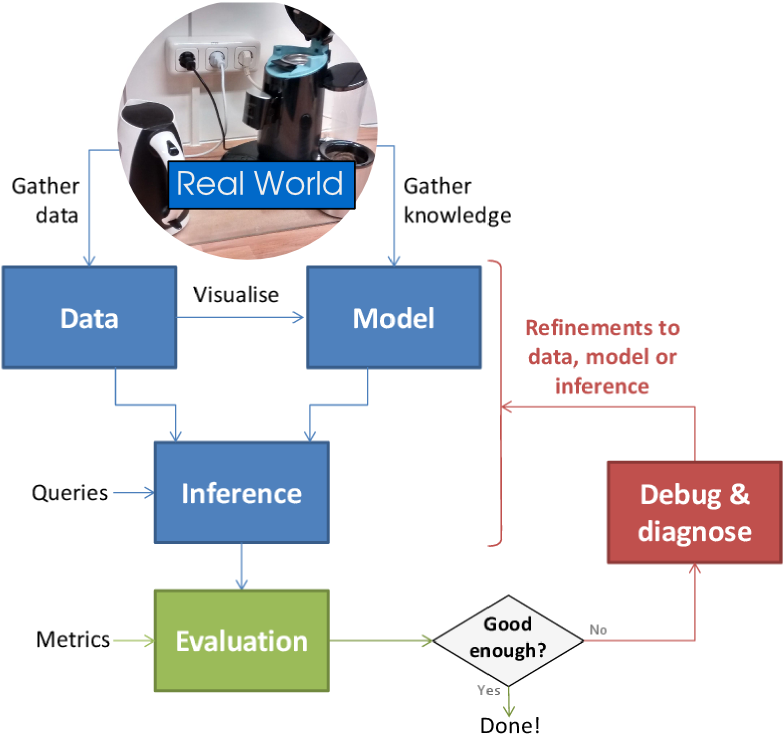
\includegraphics[scale=0.45]{pictures/location_of_object.png}
\caption{Related Work Overview}
\label{Related Work}
\end{figure}

Robots in a human-centric indoor environment need continuous interaction with the environment. The robots need to have relevant information about the objects in the environment. As a result major chunk of the research in robotics has been in this problem of searching for objects in the environment.
We start with a comprehensive treatment of the early and current work related to the object location modelling scenario that is considered in this work. This allows us to show how our work fits into this and how it pushes the state of the art.

For the purpose of clarity the literature is divided into the following categories mainly : 
\begin{itemize}
	\item Object location of novel objects 
	\item Object location of partially known objects
	\item Object location of already known non-stationary objects
\end{itemize}
\subsection{Novel objects}
\label{sub:novel objects}
In all these works the robot has no previous knowledge about the environment and instead relied on prior information of generic indoor spaces or heuristics based exploration strategy to search for novel objects. 
In the seminal paper, Bajcsy introduced the term active perception \cite {bajcsy1988active}. The focus was to move from just perceiving to searching while perceiving.

\cite{wixson1994using} recognized that searching indirectly for 'intermediate' objects can make search more efficient and provided qualitative results by comparing two search strategies. This work inspired many such other search strategies and were called as "Indirect Object Search". 

In a series of papers \cite{aydemir_plan-based_2011} \cite{aydemir_exploiting_2012}and others in the CogX project 
extended the indirect object search by introducing spatial relations to define object targets relative to landmarks.

\cite{kunze_indirect_2014} extended this approach by using probabilistic models of qualitative spatial relations to improve the object search task.
The most recent work in \textbf{Active Visual Search Problem(AVS)} is by \cite{aydemir_active_2013}, in which they have provided an comprehensive overview of the field. This work combines semantic information about the object and environment to derive better search strategy. They have compared their approach to all the existing AVS search strategies.
% subsection novel objects (end)

\subsection{Partially known objects}
\label{sub:partially known objects}
Object contextual information for searching objects as been repeatedly proven good results. Many search strategies involving searching based on known object locations have been developed
\cite{kollar_utilizing_2009} utilize object-object and object-place co-occurrences probabilities as a way to shape the prior on the object location over the search space. Using prior map of the environment and knowledge about some of the objects in it, they try to search for location of novel objects.
Extension to this approach involving information retrieval from the web has been explored by \cite {samadi_using_2012}
\cite{kunze_searching_2012} applied the semantic similarity measure for object search by using prior information from a web-trained ontology.
Finally, \cite{joho_learning_2011} illustrated one way of combining both types of information by extracting features to train a reactive search heuristics.

\cite{wong_using_2014} considered the case of occluded objects. Occluding objects in the front typically need to be moved away to enable further perception and eventual discovery of such occluded objects. 
% subsection partially known objects (end)

\subsection{Known Non-stationary Objects}
\label{sub:known non-stationary objects}
For successful execution of task for mobile-manipulation robots, should have a estimate of the state of the environment. \cite{elfring_semantic_2013} have addressed this problem by creating a model based object tracking framework. It tracks objects in the environment by modelling the uncertainty in the object location.
\cite{wong_manipulation-based_2013} have proposed a world model representation based on the objects. 
\cite{krajnik_wheres_2015}  propose a novel  approach  to  mobile  robot
search  for  non-stationary  objects  in known  environments. They use spatio temporal models for object locations .
This approach, forms the baseline for comparison of our models. Its the only approach in which long-term data from a single environment is used to make analysis of the object locations. They argue that the  probability of object occurrences at particular locations is function of time.


% subsection known non-stationary objects (end)

\subsection{User Preferences}
\label{sub:user preference}
Researchers have tried to figure out the challenges which will be involved in
placing robots in a human environment.\cite{pantofaru_exploring_2012} conducts
interviews with people to understand the needs of people with robots. One of the
suggestion was help in organizing things based on the user preferences.
For understanding user preferences in organizing objects in home work has 
been done by  \cite{abdo_collaborative_2014}, where robots learn about user
preferences in organizing objects. The learning uses data collected by 
crowdsourced data collected from thousands of users to predict location of 
novel objects. Our work differs from above as we only use data collected from a single home and predict object locations for the same home. Thus the learning is to understand and reason about a single home and not about a generalized home.

% subsection user preference (end)

% section Related Work (end)

\section{Contribution}
\label{sec:contri}
Most of the related work till now has concentrated on predicting object location for a generalized home. The data is collected for different homes together and then learning is applied generally for all homes collectively.  This work will contribute towards learning object locations for a specific home. It will do data collection in a single home and create predictions for the same. The model will thus capture the user preferences in the usage of space.

The approach proposes a way of integrating data of object location captured at
different times and locations into a dynamic spatio-temporal model and uses the
model to predict the future location of the objects. The proposed model will be
able to learn, predict, observe, relearn and refine the object locations which
enables efficient object search.


% section contri (end)
